%空行代表重启一个段落。
%开始插入附录
%\appendix
\chapter{附录I\quad 本研究所用部分载体的图谱}\label{appen:I}
%直接在奇数页页眉中显示章标题会多处一些章标题内部编号,这里重新定义\leftmark,后续所有章节都要重新定义
\renewcommand{\leftmark}{附录I\quad 本研究所用部分载体的图谱}
%将章节号计数器设置为9
\setcounter{chapter}{9}
%将插图序号计数器设置为1
\setcounter{figure}{0}
%将表格序号计数器设置为1
\setcounter{table}{0}
%开始图片浮动体环境,其中!表示取消严谨限制,h表示在此处插入,t表示在本页或下一页顶部插入
\begin{figure}[!ht]
%居中对齐
\centering
%设置图片搜索路径,每个路径用{}括起来
\graphicspath{{figures/}}
%插入图片并设置图片宽度为文本宽度减10mm
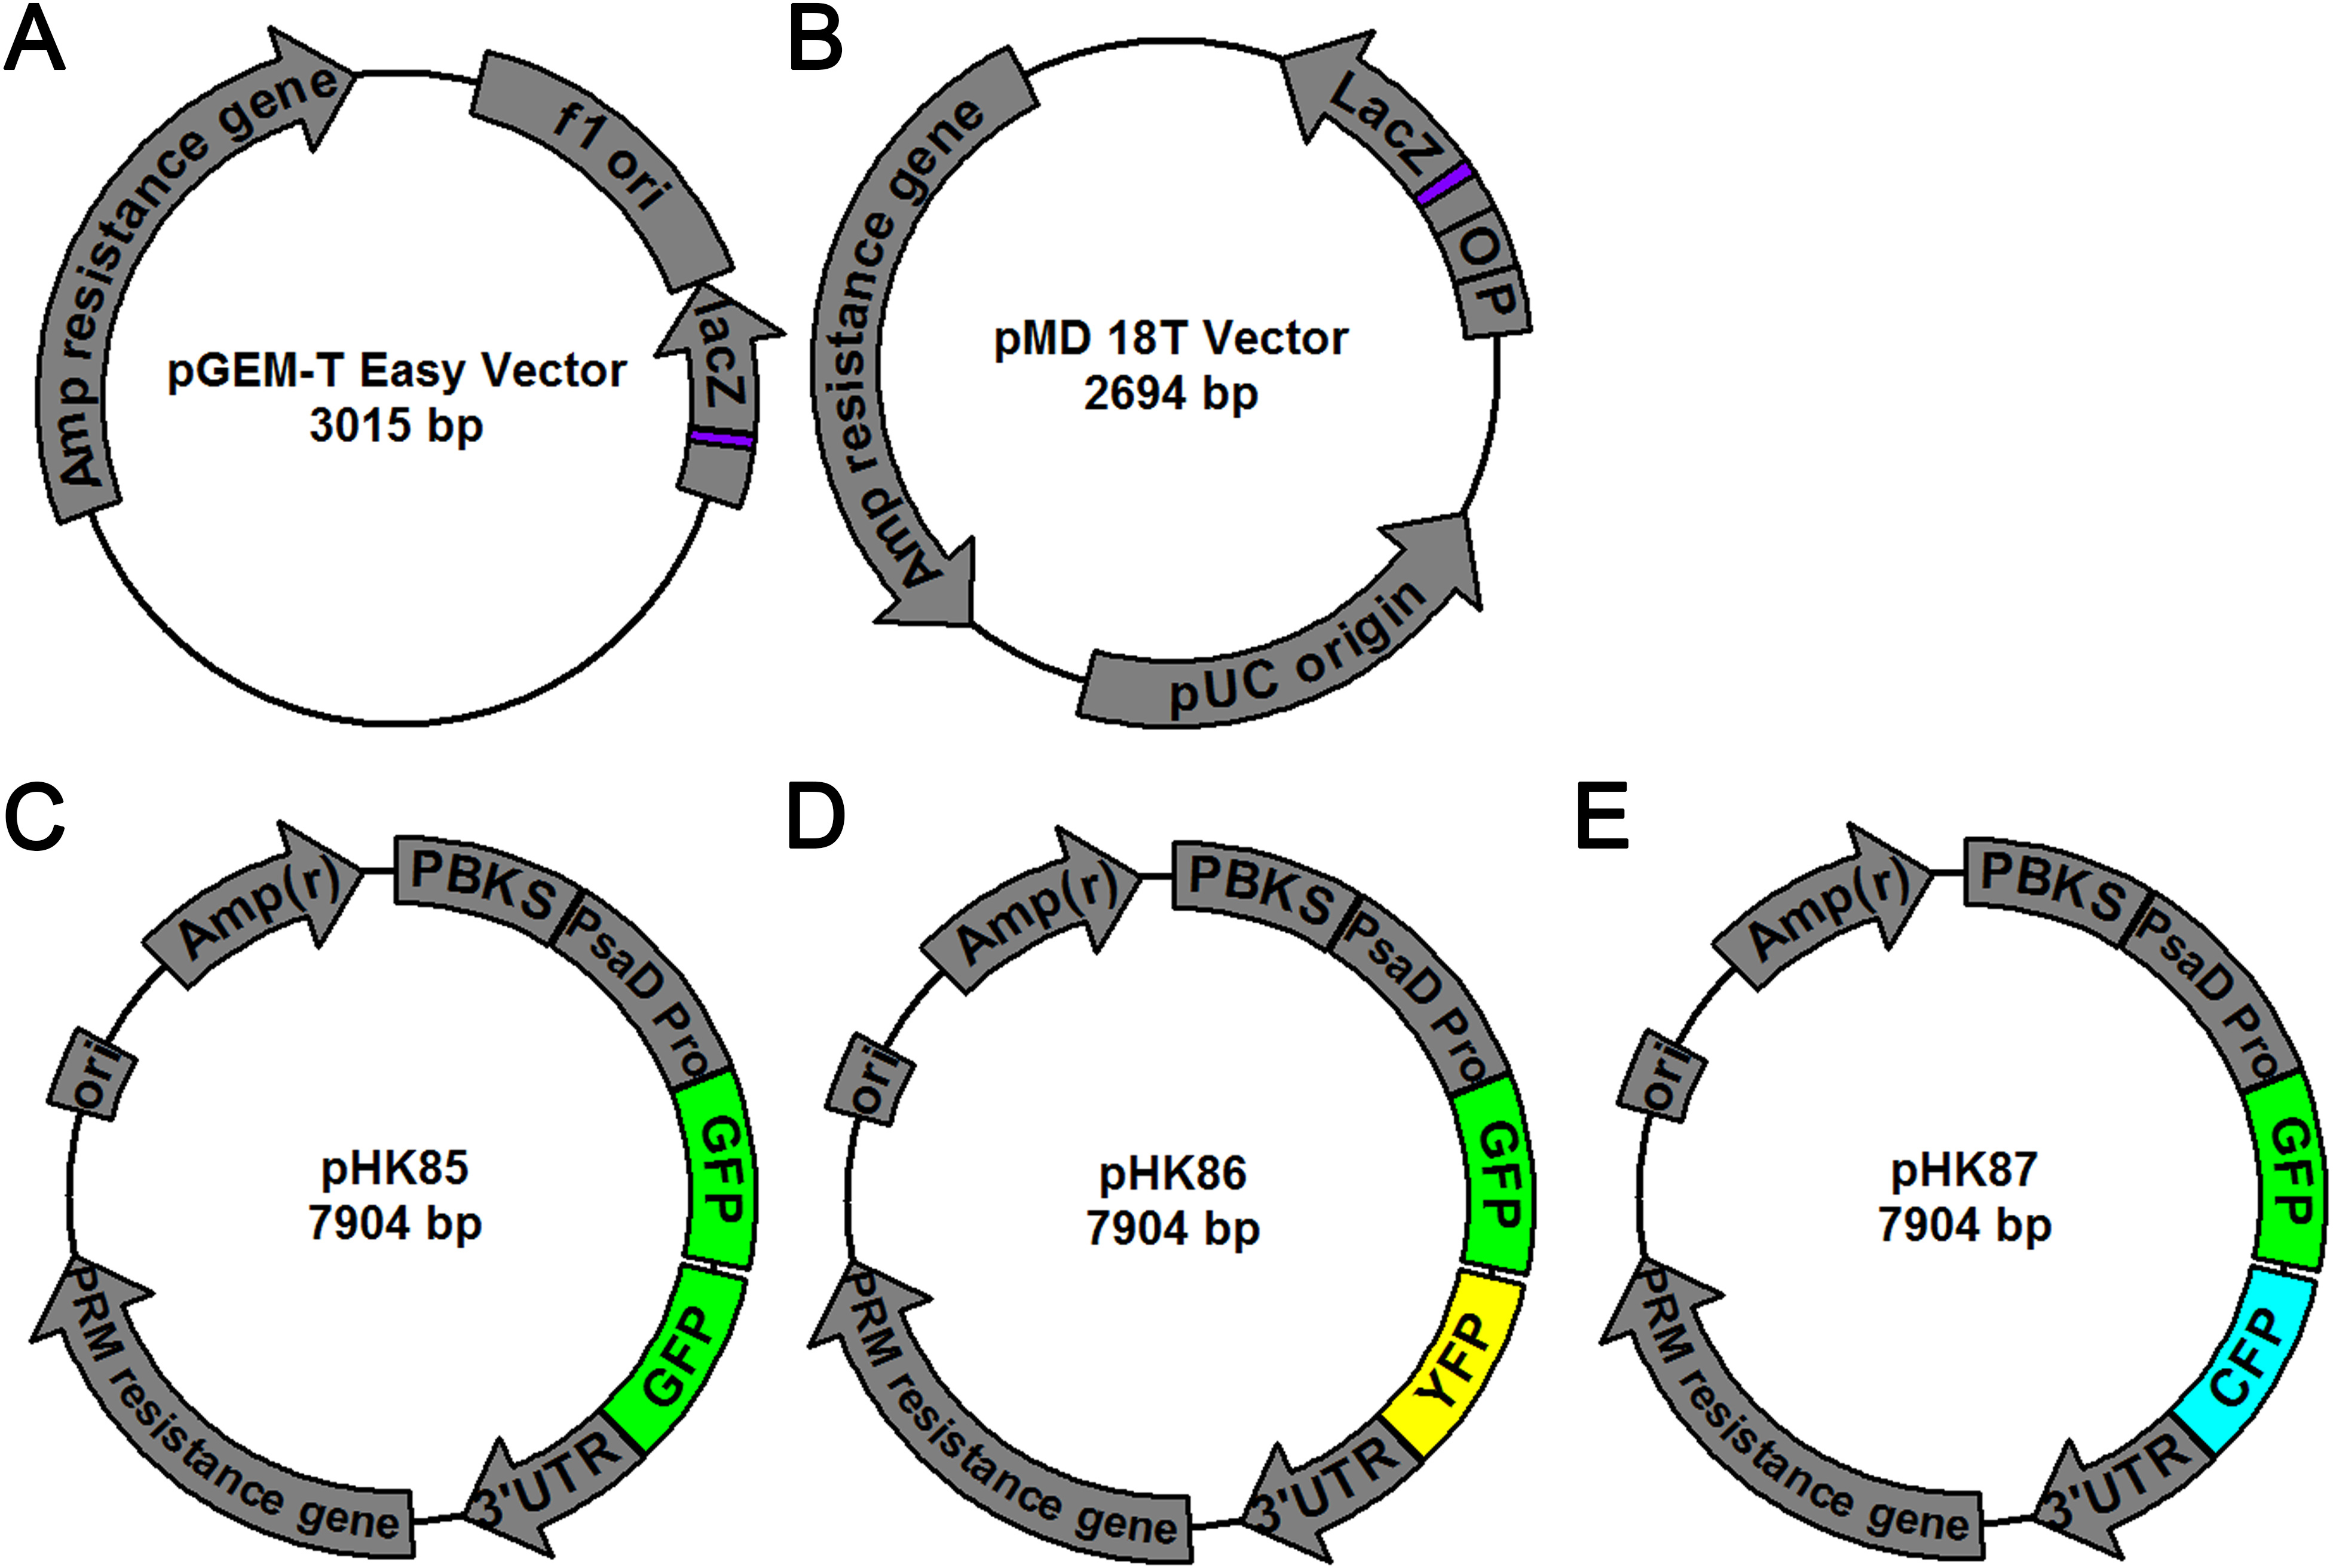
\includegraphics[width=\textwidth]{figI.jpg}
%生成中英双语标题
\bicaption[fig:I]{}{本研究所用部分载体的图谱。(A)pGEM-T Easy\ 的载体图谱。(B)pMD 18T\ 的载体图谱。(C)pHK85\ 的载体图谱。(D)pHK86\ 的载体图谱。(E)pHK87\ 的载体图谱。在\ C、D\ 和\ E\ 中,GFP\ 代表绿色荧光蛋白,YFP\ 代表黄色荧光蛋白,CFP\ 代表青色荧光蛋白。所有载体图谱均
使用\ pDRAW32\protect\footnotemark\ 绘制。在所有载体图谱中,Amp\ 代表氨苄青霉素,PRM\ 代表巴龙霉素,r\ 代表这是一个对应抗生素的抗性基因。}{Figure}{Plasmid map of some vectors constructed in this study. (A) The plasmid map of pGEM-T Easy. (B) The plasmid map of pMD 18T. (C) The plasmid map of pHK85. (D) The plasmid map of pHK86. (E) The plasmid map of pHK87. In panel C, D, and E, GFP is the green fluorescent protein. YFP represents yellow fluorescent protein. CFP indicates cyan fluorescent protein. All plasmid maps are drawn with pDRAW32. In all panels, Amp means Ampicillin. PRM is the abbreviation of paromomycin. The letter r means it is a antibiotic resistance gene.}
%结束图片浮动体环境
\end{figure}
\footnotetext{http://acaclone.com/}  